


#### Key Concepts in Predictive Models}

#### Steps in building a prediction}
\begin{enumerate}
* Find the right data
* Define your error rate
* Split data into:

* Training Set
* Testing Set
* Validation Set(optional)
<p>
* On the training set pick features
* On the training set pick prediction function
* On the training set cross-validate

* If no validation - apply 1x to test set
* If validation - apply to test set and refine
* If validation - apply 1x to validation
\end{enumerate}
%-------------------------------------------------------%

#### Type III Errors}


* Type III error is related to hypotheses suggested by the data, if tested using the data set that suggested them, are likely to be accepted even when they are not true. 

* This is because circular reasoning would be involved: something seems true in the limited data set, therefore we hypothesize that it is true in general, therefore we (wrongly) test it on the same limited data set, which seems to confirm that it is true. 

* Generating hypotheses based on data already observed, in the absence of testing them on new data, is referred to as post hoc theorizing.


* The correct procedure is to test any hypothesis on a data set that was not used to generate the hypothesis.
<p>
%-------------------------------------------------------%

#### Binary Classification}
\subsubsection*{Defining true/false positives}
In general, Positive = identified and negative = rejected. Therefore:


* True positive = correctly identified

* False positive = incorrectly identified

* True negative = correctly rejected

* False negative = incorrectly rejected
<p>
\subsubsection*{Medical testing example:}

* True positive = Sick people correctly diagnosed as sick

* False positive= Healthy people incorrectly identified as sick

* True negative = Healthy people correctly identified as healthy

* False negative = Sick people incorrectly identified as healthy.
<p>


#### Definitions}
\textbf{Accuracy Rate}\\
The accuracy rate calculates the proportion ofobservations being allocated to the \textbf{correct} group by the predictive model. It is calculated as follows:
\[ \frac{
\mbox{Number of Correct Classifications }}{\mbox{Total Number of Classifications }} \]

In the case of Binary Outcomes:
\[ = \frac{TP + TN}{TP+FP+TN+FN}\]


 \textbf{Misclassification Rate}\\
The misclassification rate calculates the proportion ofobservations being allocated to the \textbf{incorrect} group by the predictive model. It is calculated as follows:
\[ \frac{
\mbox{Number of Incorrect Classifications }}{\mbox{Total Number of Classifications }} \]
In the case of Binary Outcomes:
\[ = \frac{FP + FN}{TP+FP+TN+FN}\]







%-------------------------------------------------------%
#### Olive Oil Example}

Load the olive oil data using the commands:

```{r}
install.packages("pgmm")
library(pgmm)
data(olive)
olive = olive[,-1]
```

 These data contain information on 572 different Italian olive oils from multiple regions in Italy. 

 \textit{(Areas: (1) North Apulia, (2) Calabria, (3) South Apulia, (4) Sicily, (5) Inland Sardinia, (6) Coastal Sardinia, (7) East Liguria, (8) West Liguria, and (9) Umbria)}
```{r}
> table(olive$Area)

  1   2   3   4   5   6   7   8   9 
 25  56 206  36  65  33  50  50  51
```
 Fit a classification tree where \textbf{Area} is the outcome variable.
Then predict the value of area for the following data frame using the tree
command with all defaults.




```{r}
library(tree)
head(olive)
```

```{r}
> head(olive)
  Area Palmitic Palmitoleic Stearic Oleic Linoleic Linolenic
1    1     1075          75     226  7823      672        36
2    1     1088          73     224  7709      781        31
3    1      911          54     246  8113      549        31
4    1      966          57     240  7952      619        50
5    1     1051          67     259  7771      672        50
6    1      911          49     268  7924      678        51
  Arachidic Eicosenoic
1        60         29
2        61         29
3        63         29
4        78         35
5        80         46
6        70         44
```
The following code shows how to fit a regression tree using the \texttt{tree()} command. Area is the outcome variable, using all the other variables as predictor variables.

```{r}
olive.tree <- tree(Area ~ Palmitic + 
     Palmitoleic + Stearic + Oleic + Linoleic + 
     Linolenic + Arachidic + Eicosenoic, 
     data=olive)
```




```{r}
plot(olive.tree)
text(olive.tree)

newdata = as.data.frame(t(colMeans(olive)))

predict(olive.tree, newdata)

```

\begin{figure}
\centering
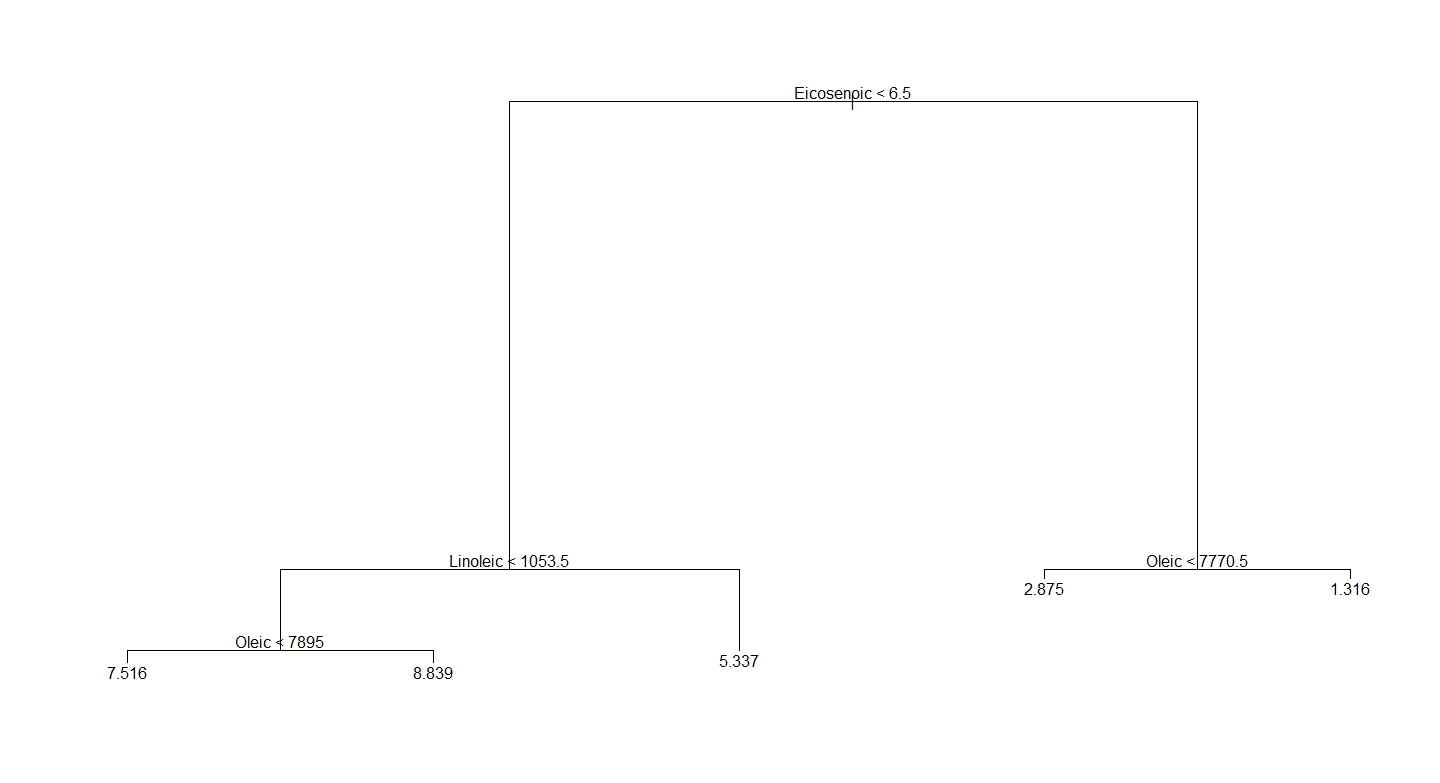
\includegraphics[width=0.70\linewidth]{./DAquiz6q4a}
\caption{}
\label{fig:DAquiz6q4a}
\end{figure}
\subsection*{Answer}
2.875. It is strange because Region should be a qualitative variable - but tree is reporting the average value of Region as a numeric variable in the leaf predicted for newdata.


%-------------------------------------------------------%
\subsection*{Question 5}
Suppose that I fit and prune a tree to get the following diagram. What area
would I predict for a new value of:

```{r}
olive.tree <- tree(as.factor(Area) ~ Palmitic + 
         Palmitoleic + Stearic + Oleic + Linoleic + 
         Linolenic + Arachidic + Eicosenoic, data=olive)

plot(olive.tree); text(olive.tree)
```

\begin{figure}[h!]
\centering
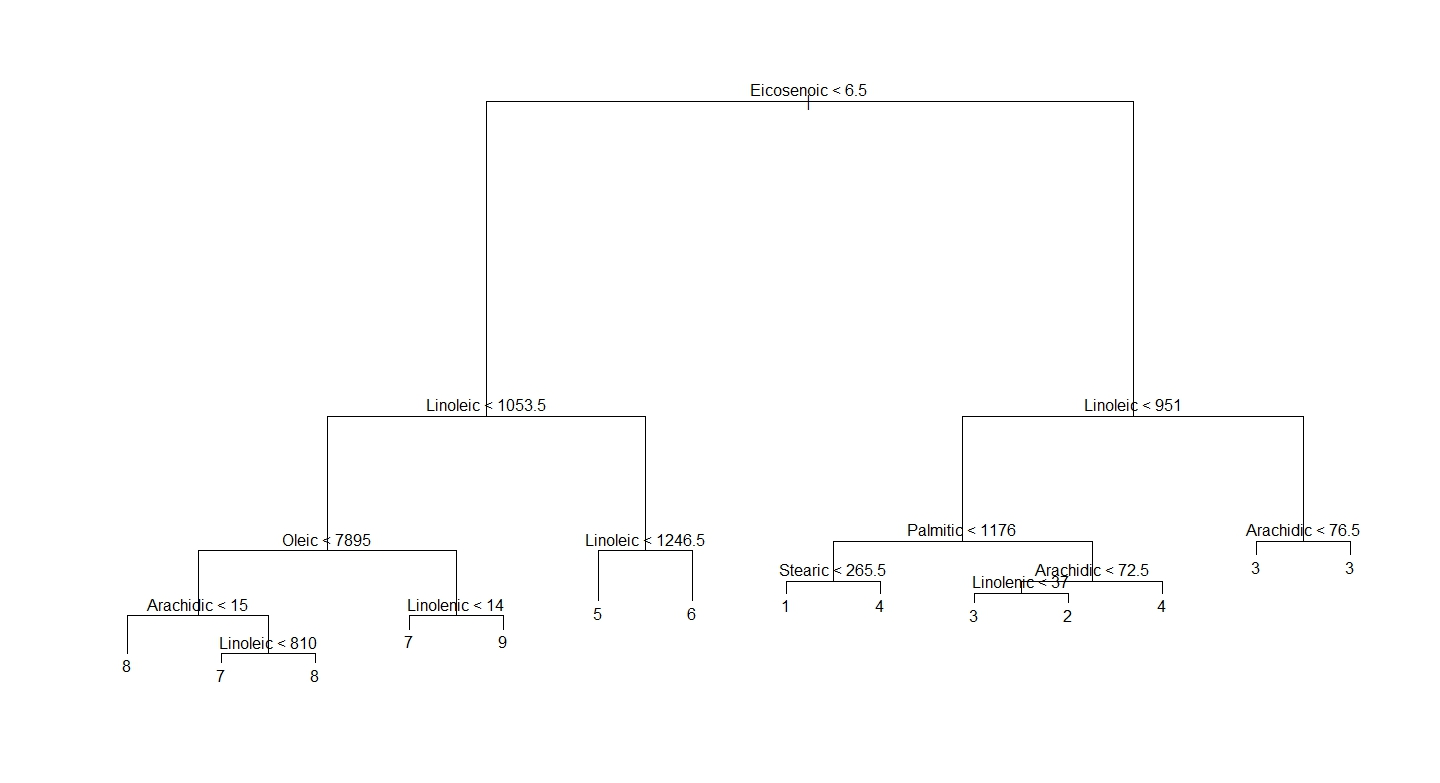
\includegraphics[width=1.19\linewidth]{./DAquiz6q5a}
\caption{}
\label{fig:DAquiz6q5a}
\end{figure}

%----------------------------------------------------------------------------------------------%
<h4>Tree Pruning}
% Is this revelant to caret?
The \texttt{prune.tree()} command determines a nested sequence of subtrees of the supplied tree by recursively “snipping” off the least important splits in the regression tree.

```{r}
olive.pruned <- prune.tree(olive.tree,best=6)

plot(olive.pruned); text(olive.pruned)
```

\begin{figure}[h!]
\centering
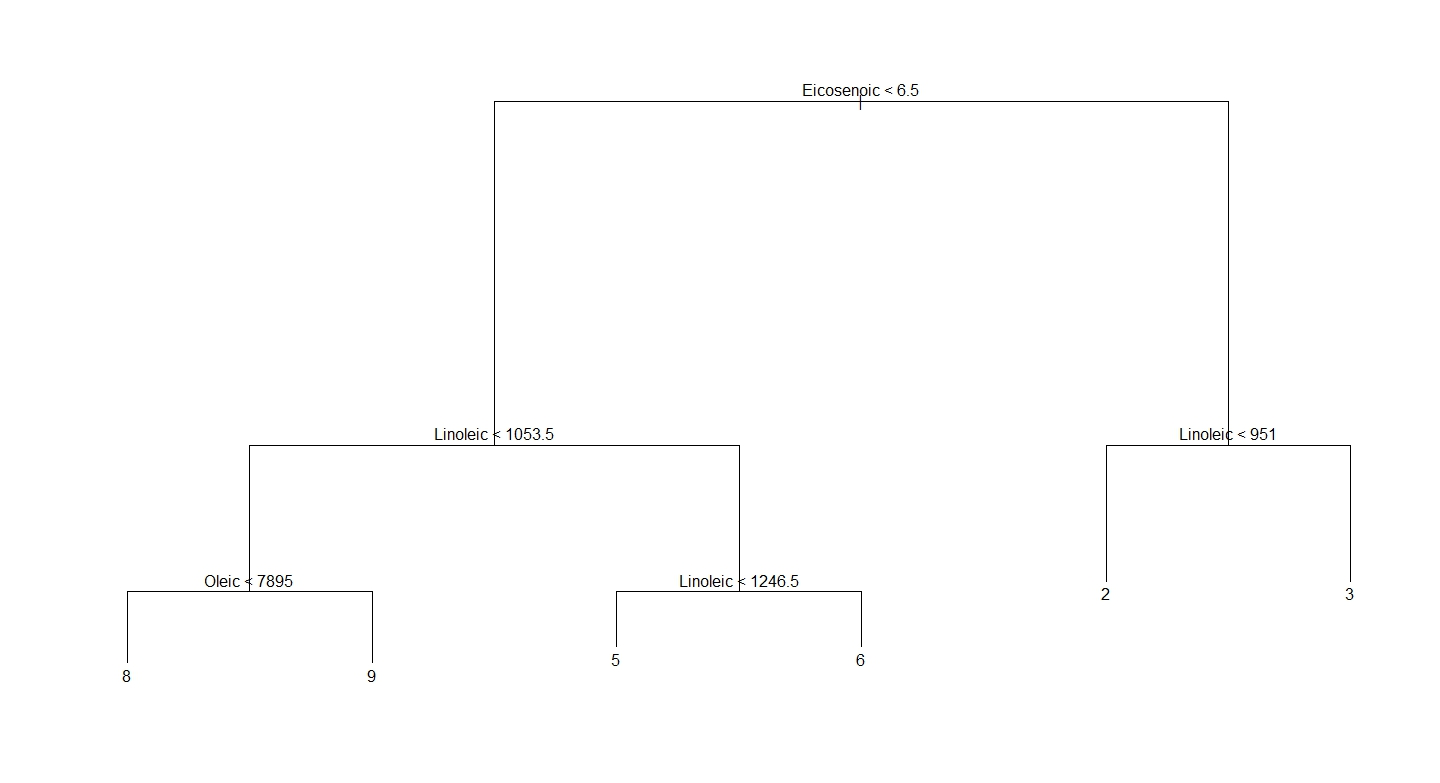
\includegraphics[width=1.19\linewidth]{./DAquiz6q5b}
\caption{}
\label{fig:DAquiz6q5b}
\end{figure}


```{r}
newData = data.frame(Palmitic = 1200, Palmitoleic = 120, 
          Stearic=200, Oleic=7000, Linoleic = 900, 
          Linolenic = 32, Arachidic=60, Eicosenoic=6)

predict(olive.pruned, newData)
```


```{r}
predict(olive.pruned, newData)
  1 2 3 4 5 6         7         8 9
1 0 0 0 0 0 0 0.4842105 0.5157895 0
```
<p>
